\usetikzlibrary{quotes} 
% the `quotes` library for adding annotations with an easy quoting syntax that 
% we will use in the drawing
\documentclass[tikz,border=10pt]{standalone} % 
% the `standalone` document class allows us to create documents that consist
% only of a single drawing and cuts the PDF document to the actual content
% \usepackage{tikz} is not needed if [tikz] is set
\begin{document}
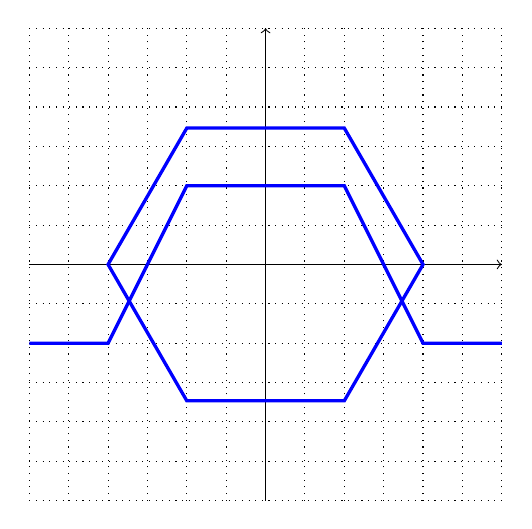
\begin{tikzpicture}
	% \draw[<style>] <coordinate> <picture element> <coordinate> ...;
	% \draw produces a path with coordinates and picture elements in between
	% until we end with a semicolon
	\draw[thin,dotted,step=0.5] (-3,-3) grid (3,3);
	\draw[->] (-3,0) -- (3,0);
	% -- for line
	% -> for arrow
	\draw[->] (0,-3) -- (0,3);
	\draw[very thick, blue] (0:2) -- (60:2) -- (120:2)
    -- (180:2) --(240:2) -- (300:2) -- cycle;
	% TikZ uses a distinguish it form Cartesian coordinates in ploar coordinate
	% system (angle:distance)
    \draw[very thick, blue] (-3,-1) -- ++(1,0) -- ++(1,2) -- ++(2,0) --++ (1,-2) -- ++ (1,0);
	% + relative position to the first coordinate
	% ++ double plus sign

\end{tikzpicture}

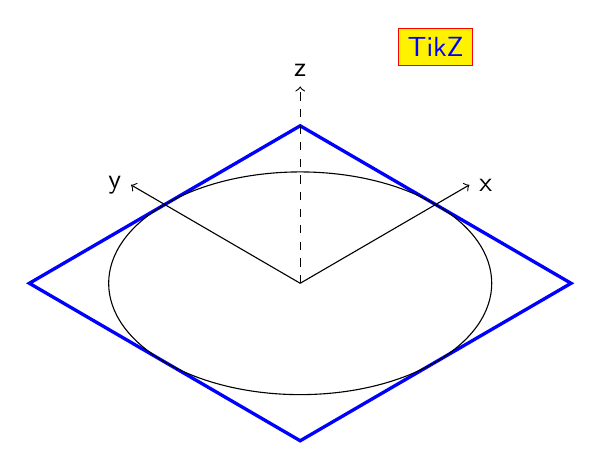
\begin{tikzpicture}[y={(-0.86cm,0.5cm)},x={(0.86cm,0.5cm)}, z={(0cm,1cm)},font=\sffamily]
  \draw[very thick, blue] (-2,-2,0) -- (-2,2,0) -- (2,2,0) -- (2,-2,0) -- cycle;
  \draw[->] (0,0,0) -- (2.5, 0,  0) node [right] {x};
  \draw[->] (0,0,0) -- (0,  2.5, 0) node [left] {y};
  \draw[->,dashed] (0,0,0) -- (0,  0, 2.5) node [above] {z};
  \draw circle (2);
  \draw (4, 2) node[draw, color = red, fill = yellow, text = blue] {TikZ}; 
  % [draw] draw the border
\end{tikzpicture}

\end{document}

